\documentclass[11pt]{article}
% Shared preamble for the NSE working-paper series (Mrigank Sahi).
% Usage in each paper: % Shared preamble for the NSE working-paper series (Mrigank Sahi).
% Usage in each paper: % Shared preamble for the NSE working-paper series (Mrigank Sahi).
% Usage in each paper: \input{../common/preamble.tex}
\usepackage[T1]{fontenc}
\usepackage[utf8]{inputenc}
\usepackage{lmodern}
\usepackage{microtype}
\usepackage[a4paper,margin=1in]{geometry}
\usepackage{amsmath,amssymb}
\usepackage{booktabs}
\usepackage{tabularx}
\usepackage{siunitx}
\sisetup{group-separator={,},round-mode=places,round-precision=3}
\usepackage{graphicx}
\usepackage{xcolor}
\usepackage{caption}
\captionsetup{font=small,labelfont=bf}
\usepackage{enumitem}
\setlist{nosep,leftmargin=*}
\usepackage[framemethod=TikZ]{mdframed}
\usepackage[numbers,sort&compress]{natbib}
\usepackage[colorlinks=true,linkcolor=black,citecolor=blue!50!black,urlcolor=blue!50!black]{hyperref}

\newcommand{\ghbase}{https://github.com/mriganksahi-beep}
\newcommand{\authorline}{Mrigank Sahi\\\small Independent Researcher, New Delhi\\\small\texttt{mriganksahi@gmail.com}}

% Standard disclosure box. Every paper fills all five fields.
% #1 sample/period status, #2 position in test tally, #3 costs,
% #4 point-in-time limits, #5 anything else the reader must know
\newcommand{\caveatsbox}[5]{%
\begin{mdframed}[backgroundcolor=gray!8,linecolor=gray!50,innertopmargin=6pt,innerbottommargin=6pt]
\small\textbf{Read before interpreting results.}
\begin{itemize}
\item \textbf{Sample.} #1
\item \textbf{Multiple testing.} #2
\item \textbf{Costs.} #3
\item \textbf{Point-in-time universe.} #4
\item \textbf{Other.} #5
\end{itemize}
\end{mdframed}}

% Standard AI-assistance statement (identical across the series).
\newcommand{\aistatement}{%
\paragraph{Use of AI tools.} Code for this project was written with the assistance of
an AI coding assistant (Anthropic's Claude), working to specifications set by the
author, and the manuscript was drafted with the same assistance. The author designed
the research questions and decision rules and ran the main analyses. Some diagnostics
added during revision were computed by the assistant from archived run outputs; these
are labelled as revision diagnostics in the text. The author reviewed all code and
text and takes full responsibility for the content.}

% Standard data/code availability statement.
\newcommand{\availability}[1]{%
\paragraph{Data and code availability.} Code: \url{#1}. The point-in-time panel
construction is documented in \url{\ghbase/indian-equity-research/tree/main/data_pipeline}.
Price data from Yahoo Finance and index-membership snapshots from a licensed vendor
are not redistributed; the repository contains the scripts to rebuild the panel.}

% Placeholder for anything awaiting the author's confirmation. Renders red so it
% cannot survive into a posted PDF unnoticed.
\newcommand{\verify}[1]{\textcolor{red}{\textbf{[VERIFY: #1]}}}

\usepackage[T1]{fontenc}
\usepackage[utf8]{inputenc}
\usepackage{lmodern}
\usepackage{microtype}
\usepackage[a4paper,margin=1in]{geometry}
\usepackage{amsmath,amssymb}
\usepackage{booktabs}
\usepackage{tabularx}
\usepackage{siunitx}
\sisetup{group-separator={,},round-mode=places,round-precision=3}
\usepackage{graphicx}
\usepackage{xcolor}
\usepackage{caption}
\captionsetup{font=small,labelfont=bf}
\usepackage{enumitem}
\setlist{nosep,leftmargin=*}
\usepackage[framemethod=TikZ]{mdframed}
\usepackage[numbers,sort&compress]{natbib}
\usepackage[colorlinks=true,linkcolor=black,citecolor=blue!50!black,urlcolor=blue!50!black]{hyperref}

\newcommand{\ghbase}{https://github.com/mriganksahi-beep}
\newcommand{\authorline}{Mrigank Sahi\\\small Independent Researcher, New Delhi\\\small\texttt{mriganksahi@gmail.com}}

% Standard disclosure box. Every paper fills all five fields.
% #1 sample/period status, #2 position in test tally, #3 costs,
% #4 point-in-time limits, #5 anything else the reader must know
\newcommand{\caveatsbox}[5]{%
\begin{mdframed}[backgroundcolor=gray!8,linecolor=gray!50,innertopmargin=6pt,innerbottommargin=6pt]
\small\textbf{Read before interpreting results.}
\begin{itemize}
\item \textbf{Sample.} #1
\item \textbf{Multiple testing.} #2
\item \textbf{Costs.} #3
\item \textbf{Point-in-time universe.} #4
\item \textbf{Other.} #5
\end{itemize}
\end{mdframed}}

% Standard AI-assistance statement (identical across the series).
\newcommand{\aistatement}{%
\paragraph{Use of AI tools.} Code for this project was written with the assistance of
an AI coding assistant (Anthropic's Claude), working to specifications set by the
author, and the manuscript was drafted with the same assistance. The author designed
the research questions and decision rules and ran the main analyses. Some diagnostics
added during revision were computed by the assistant from archived run outputs; these
are labelled as revision diagnostics in the text. The author reviewed all code and
text and takes full responsibility for the content.}

% Standard data/code availability statement.
\newcommand{\availability}[1]{%
\paragraph{Data and code availability.} Code: \url{#1}. The point-in-time panel
construction is documented in \url{\ghbase/indian-equity-research/tree/main/data_pipeline}.
Price data from Yahoo Finance and index-membership snapshots from a licensed vendor
are not redistributed; the repository contains the scripts to rebuild the panel.}

% Placeholder for anything awaiting the author's confirmation. Renders red so it
% cannot survive into a posted PDF unnoticed.
\newcommand{\verify}[1]{\textcolor{red}{\textbf{[VERIFY: #1]}}}

\usepackage[T1]{fontenc}
\usepackage[utf8]{inputenc}
\usepackage{lmodern}
\usepackage{microtype}
\usepackage[a4paper,margin=1in]{geometry}
\usepackage{amsmath,amssymb}
\usepackage{booktabs}
\usepackage{tabularx}
\usepackage{siunitx}
\sisetup{group-separator={,},round-mode=places,round-precision=3}
\usepackage{graphicx}
\usepackage{xcolor}
\usepackage{caption}
\captionsetup{font=small,labelfont=bf}
\usepackage{enumitem}
\setlist{nosep,leftmargin=*}
\usepackage[framemethod=TikZ]{mdframed}
\usepackage[numbers,sort&compress]{natbib}
\usepackage[colorlinks=true,linkcolor=black,citecolor=blue!50!black,urlcolor=blue!50!black]{hyperref}

\newcommand{\ghbase}{https://github.com/mriganksahi-beep}
\newcommand{\authorline}{Mrigank Sahi\\\small Independent Researcher, New Delhi\\\small\texttt{mriganksahi@gmail.com}}

% Standard disclosure box. Every paper fills all five fields.
% #1 sample/period status, #2 position in test tally, #3 costs,
% #4 point-in-time limits, #5 anything else the reader must know
\newcommand{\caveatsbox}[5]{%
\begin{mdframed}[backgroundcolor=gray!8,linecolor=gray!50,innertopmargin=6pt,innerbottommargin=6pt]
\small\textbf{Read before interpreting results.}
\begin{itemize}
\item \textbf{Sample.} #1
\item \textbf{Multiple testing.} #2
\item \textbf{Costs.} #3
\item \textbf{Point-in-time universe.} #4
\item \textbf{Other.} #5
\end{itemize}
\end{mdframed}}

% Standard AI-assistance statement (identical across the series).
\newcommand{\aistatement}{%
\paragraph{Use of AI tools.} Code for this project was written with the assistance of
an AI coding assistant (Anthropic's Claude), working to specifications set by the
author, and the manuscript was drafted with the same assistance. The author designed
the research questions and decision rules and ran the main analyses. Some diagnostics
added during revision were computed by the assistant from archived run outputs; these
are labelled as revision diagnostics in the text. The author reviewed all code and
text and takes full responsibility for the content.}

% Standard data/code availability statement.
\newcommand{\availability}[1]{%
\paragraph{Data and code availability.} Code: \url{#1}. The point-in-time panel
construction is documented in \url{\ghbase/indian-equity-research/tree/main/data_pipeline}.
Price data from Yahoo Finance and index-membership snapshots from a licensed vendor
are not redistributed; the repository contains the scripts to rebuild the panel.}

% Placeholder for anything awaiting the author's confirmation. Renders red so it
% cannot survive into a posted PDF unnoticed.
\newcommand{\verify}[1]{\textcolor{red}{\textbf{[VERIFY: #1]}}}

\usepackage{xurl}
\newcommand{\miex}{\mathrm{MI}_{\mathrm{excess}}}

\title{\textbf{Mutual Information in the Cross-Section of Indian Equities:\\
Sign Instability, Feature Overlap, and Conditional-MI Calibration}}
\author{\authorline}
\date{October 2026}

\begin{document}
\maketitle

\begin{abstract}
\noindent
I screen six price- and volume-based features against forward returns at five
horizons in a snapshot-based point-in-time Nifty~500 universe, 2010--2021, using a
rank-based mutual information (MI) estimator with a within-date permutation null.
All 30 feature--horizon cells have permutation-corrected MI above zero at nominal
95\% moving-block bootstrap intervals, and all 30 survive a Holm family-wise
adjustment. Only 13 have a mean rank information coefficient (IC) that survives the
same adjustment. Most of the gap is not hidden nonlinearity. Much of the measured
information comes from monotone relationships that are strong in a given month but
change sign across months; an averaged IC cancels these, and sign-blind MI does not.
Between features, MI is most informative where rank correlation is weakest: reversal
and momentum are each U-shaped in volatility. A first conditional-MI analysis
reported synergy for every pair tested; diagnostics traced this to mixing two
estimators and a mis-specified noise benchmark, and the corrected analysis shows net
redundancy between momentum and volatility and no synergy. MI indicates whether a
feature sorts the cross-section of returns, not in which direction.
\end{abstract}

\caveatsbox
{Development period only. Rebalances run from 2010-01 to 2021-12, and every forward window ends on or before 2021-12-31 (a code guard drops any rebalance whose window would cross it; an independent audit re-checked every date used). The later period was not read.}
{The screen is a characterization; no feature or horizon was selected from it. In the project's test ledger it is family MI-33 (30 cells), with CMI-34 (four conditional-MI pairs) and MI-35 (two analyses added in the 2026 re-run). These sit after the 32 entries of the original ledger. Nominal and Holm-adjusted results are both reported.}
{No portfolios are formed and no returns are claimed; costs do not arise.}
{Index membership is a snapshot-based approximation built from semi-annual snapshots (first snapshot mid-2010). The 2018-06-30 snapshot is truncated, so membership for Jul--Dec 2018 is approximate.}
{The panel's date index contains some exchange-closed dates on which most stocks have no data. Months whose rebalance date or forward-window end fell on such a date were dropped (Section~\ref{sec:data}); a calendar-corrected re-run is planned.}

\section{Introduction}

Information coefficients, the rank correlations between a feature and forward
returns, are the standard currency for comparing cross-sectional signals. They detect
only monotone relationships with a consistent sign. Mutual information measures any
statistical dependence and is sometimes proposed as a screening tool that catches what
correlation misses. This paper asks what MI adds on Indian equity data, and what is
required to use it correctly.

I compute a permutation-corrected MI between the cross-sectional ranks of six features
(12-1 momentum, one-month reversal, 60-day realized volatility, 21-day log turnover,
21-day overnight-return tilt, and lagged Amihud illiquidity) and forward returns at
horizons from one week to one year. The answer has three parts. First, MI flags every
feature as informative, but for half the cells the information has no stable
direction: monthly rank ICs are often large in absolute value and change sign through
time. MI averages the strength of the relationship; IC averages its signed value.
Second, MI between features separates monotone overlap, which correlation already
describes, from U-shaped relationships, which it does not. Third, conditional MI is
easy to misread: a naive implementation produced an apparent synergy for every pair,
and the paper documents how that result was diagnosed and corrected.

The contribution is methodological and descriptive. It does not propose a trading
rule. Related work by the author studies regime-dependent momentum and reversal ICs in
the same market \citep{sahi_irfa}; the sign instability documented here is one reason
such conditioning is worth studying.

\section{Data and universe}
\label{sec:data}

The panel covers NSE-listed stocks from 2010-01-04 to 2026-07-10 (4,237 dates in the
panel index, 1,069 tickers), built from Yahoo Finance prices. Historical Nifty~500
membership is a snapshot-based point-in-time approximation from semi-annual index
snapshots, expanded into a daily membership flag. Construction, validation and known
data defects are documented in the panel repository (see the availability statement).

Choices specific to this paper:
\begin{itemize}
\item Only stocks with membership flag equal to 1 on the rebalance date are used.
Missing values are dropped, never filled.
\item Trailing 21-day features are averaged over each stock's own trading rows. About
31\% of (date, stock) cells in the wide panel are empty (closed dates, masked rows,
pre-listing), and a calendar window would have left these features empty for most of
the universe.
\item Amihud illiquidity \citep{amihud2002} is computed monthly and attached with a
one-month lag: a rebalance in month $M$ uses month $M-1$'s value.
\end{itemize}

Rebalance dates are the last date in each calendar month present in the panel index,
2010-01 to 2021-12 (144 dates). A date is dropped for a cell if fewer than 30 eligible
stocks remain or if its forward window would cross 2021-12-31. At the one-month
horizon, cells lose the first five months of 2010 (before the first membership
snapshot; momentum, which needs 252 rows of history, loses most of 2010), December
2021 (hold-out guard), and eleven mid-sample months: 2011-08, 2014-03, 2014-06,
2014-07, 2014-08, 2016-10, 2018-02, 2018-03, 2019-09, 2020-11 and 2021-02. Five of
these (2011-08, 2014-08, 2016-10, 2018-03 and 2020-11) end on an exchange holiday;
the panel's last date in those months appears to be the closed date, carrying data for
only a few stocks, so the rebalance cross-section collapses. The cause of the other six has not been verified; a closed
date at the end of the forward window would have the same effect. A closed date inside
a window also lengthens a row-counted horizon by one trading day. Dropping these months
removes about 8\% of dates and reduces precision; whether it shifts any estimate will
be known after the calendar-corrected re-run. Each cell retains between 97 and 129
dates with 464--490 stocks per date on average.

\section{Method}

\subsection{Permutation-corrected mutual information}
On each rebalance date $t$, the feature and the $h$-day forward return are converted
to cross-sectional ranks scaled to $(0,1)$. Ranking removes date-level changes in the
location and scale of returns, including the common market move, and makes the
analysis invariant to monotone transformations; it does not remove differences in
stocks' exposures to the market or to other factors. MI between the two rank vectors
is estimated with the Kraskov--St\"ogbauer--Grassberger nearest-neighbour estimator
\citep{kraskov2004} ($k=3$, scikit-learn). Because this estimator is biased in finite
samples, the same quantity is recomputed after 40 random permutations of the return
ranks within the date, and
\[
\miex(t) = \widehat{\mathrm{MI}}(t) - \tfrac{1}{40}\textstyle\sum_{p=1}^{40}
\widehat{\mathrm{MI}}_{\pi_p}(t).
\]
The cell estimate is the mean of $\miex(t)$ over dates. The date is the unit of
analysis. Pooling stocks from different dates and bootstrapping the pooled sample
would place duplicate points in the nearest-neighbour search, which biases this class
of estimator upward; estimating one value per date avoids that.

\subsection{Inference}
Intervals are 95\% percentile intervals from a circular moving-block bootstrap
\citep{kunsch1989,politis1992} over the per-date series (2,000 draws). Monthly
rebalances with forward windows longer than a month overlap, so the block length is at
least the horizon: 3 months for the one-week, one-month and three-month horizons, 6 for
six months and 12 for one year. Because the 30 cells form one family, I also report a
Holm family-wise adjustment \citep{holm1979} using $z$-statistics from the bootstrap
standard errors. Mean ICs are computed per date and averaged with equal weight per
date; their intervals use the same bootstrap.

\subsection{Direction versus rank extremeness}
MI is sign-blind, so a positive $\miex$ does not say whether high-feature stocks
outperform. For every cell and date I also compute (i) the rank IC, the Spearman
correlation of feature and forward return, and (ii) an extremeness MI and
extremeness IC, obtained by replacing the forward-return rank $u$ with the rank of
$|u-0.5|$. This measures how far a stock's return rank sits from the cross-sectional
median in either direction; it is a rank-based proxy for the size of the move, not
the percentage return itself. Before the real-data run I fixed a descriptive
classification for each cell: \emph{no signal} if the $\miex$ interval includes zero;
\emph{extremeness-led} if extremeness MI is at least half of $\miex$ and its interval
excludes zero; \emph{direction-led} if that share is below half and the IC interval
excludes zero; otherwise \emph{mixed}. The one-half cut-off is a convention, not a
test; the class labels are a taxonomy for reading Figure~\ref{fig:landscape}.

To compare MI with rank correlation on one scale, each date's Spearman $\rho$ is
converted into the MI of a Gaussian copula with that rank correlation,
$-\tfrac12\ln(1-r^2)$ with $r = 2\sin(\pi\rho/6)$, minus its expected value under
independence at that date's cross-section size, $\tfrac12(\pi/3)^2/(n-1)$. A
simulation confirmed that this correction averages zero under independence. The
conversion is an approximation, used only for comparisons.

\subsection{Conditional mutual information}
To ask whether feature $A$ carries information about returns $Y$ beyond feature $B$,
I estimate $I(A;Y\mid B)$ per date with a nearest-neighbour conditional estimator
(\texttt{npeet}), subtracting a within-date permutation null. Four pairs were fixed
before running, all at the one-month horizon: momentum given volatility, volatility
given momentum, reversal given momentum, and Amihud given turnover.
Section~\ref{sec:cmi} describes how the first version of this analysis failed and how
it was corrected.

\subsection{Validation gates}
No real-data run proceeded until synthetic self-tests passed: a panel with a planted
predictive feature and a pure-noise feature (planted $\miex = 0.135$; noise $0.004$,
90\% interval $[-0.002, 0.011]$); deliberate tests of the membership filter, warm-up
gaps, leakage and the hold-out guard; known-redundant and known-additive pairs for the
conditional estimator; and, for the 2026 re-run, planted direction-only and
volatility-only features for the classification rule.

\section{Results}

\subsection{Every feature is informative; about half have a stable direction}

\begin{figure}[t]
\centering
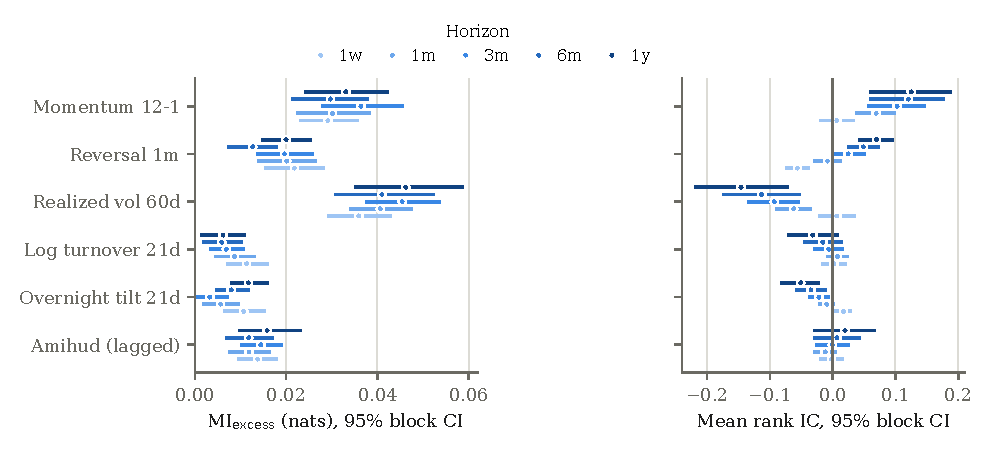
\includegraphics[width=\textwidth]{figures/fig1_landscape.pdf}
\caption{Left: permutation-corrected MI between feature rank and forward-return rank,
by horizon. Right: mean monthly rank IC for the same cells. Bars are 95\% moving-block
bootstrap intervals. All 30 MI intervals exclude zero (30 after Holm adjustment); 15 IC
intervals do (13 after Holm adjustment). Development period 2010--2021.}
\label{fig:landscape}
\end{figure}

Figure~\ref{fig:landscape} shows the landscape. All 30 $\miex$ intervals exclude zero,
and all 30 cells remain significant at the 5\% family-wise level after Holm
adjustment. Realized volatility (0.033--0.043 nats) and momentum (0.026--0.041) carry
the most information, then reversal (0.012--0.022); Amihud, turnover and overnight
tilt lie between 0.005 and 0.017. The weakest cell, overnight tilt at three months,
is fragile: its lower bound is close to zero with 3- or 6-month blocks and falls just
below zero with 12-month blocks. No other cell's conclusion depends on the block
length.

The IC panel tells a different story. Momentum has a positive mean IC from one month
onward (0.085 at one month, 95\% interval $[0.049, 0.122]$; 0.131 at six months) but
none at one week.\footnote{The momentum IC reported by \citet{sahi_momentum}, 0.061,
uses 2011--2026 and a different return harness. Restricting this paper's one-month
series to 2011--2021 gives 0.084, so the different start date does not explain the
gap; the inclusion of 2022--2026 and harness differences remain possible causes and
have not been separated.} Volatility has a negative IC that strengthens with horizon
($-0.066$ at one month, $-0.146$ at one year, $[-0.218,-0.072]$), consistent with the
low-volatility pattern documented elsewhere \citep{ang2006}. Reversal is negative at
one week ($-0.042$) and positive at six and twelve months. Turnover's and Amihud's IC
intervals include zero at every horizon; overnight tilt's IC is positive at one week
and negative from three months, and only the six- and twelve-month values survive
Holm adjustment. In total, 15 IC intervals exclude zero nominally and 13 survive Holm
adjustment. Under the descriptive classification, 13 cells are direction-led, 4
extremeness-led, 13 mixed and none without signal. Volatility carries both kinds of
information: alongside its negative IC, its extremeness IC is 0.16--0.17 at every
horizon. High-volatility stocks end further from the median, in either direction.

\subsection{Much of the information has no stable sign}

\begin{figure}[t]
\centering
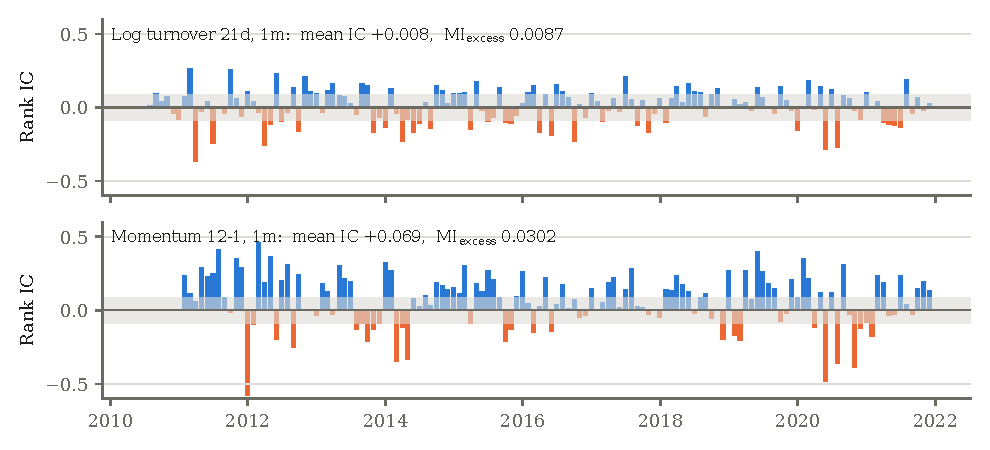
\includegraphics[width=\textwidth]{figures/fig3_ic_series.pdf}
\caption{Monthly rank IC at the one-month horizon. The grey band is
$\pm1.96/\sqrt{n-1}$, a reference for sampling noise if stocks were independent; it
is not a calibrated null, since returns are cross-sectionally correlated. Turnover's
monthly ICs fall outside the band in both directions and average to almost zero;
momentum's are mostly positive.}
\label{fig:icseries}
\end{figure}

Why do so many cells carry information without a stable direction?
Figure~\ref{fig:icseries} shows the pattern, and Table~\ref{tab:sign} quantifies it.
At one month, turnover's IC lies above the reference band in 28\% of months and below
it in 19\%, and the two cancel to a mean of $0.009$. Momentum is the contrast: 57\%
above, 16\% below. Across all 30 cells, between 28\% and 78\% of months fall outside
the band, against 5\% expected if stocks were independent and there were no
relationship. Some of this excess reflects cross-sectional correlation among stocks,
which widens the true sampling distribution of a monthly IC. A likely economic reading
is that several features are correlated with exposures to common factors or sectors
whose returns change sign from month to month; the month's association is real, but
its direction follows the factor return. This mechanism is not tested here.

\begin{table}[t]
\centering\small
\caption{One-month horizon. Share of months with IC above / below the reference band;
mean IC; and Gaussian-copula MI implied by the mean IC versus by each month's own IC
(then averaged). Negative null-corrected values are shown as $\approx0$.}
\label{tab:sign}
\begin{tabular}{lrrrrrr}
\toprule
& \multicolumn{2}{c}{Months outside band} & & \multicolumn{2}{c}{Implied MI (nats)} & \\
\cmidrule(lr){2-3}\cmidrule(lr){5-6}
Feature & above & below & Mean IC & from mean IC & from monthly IC & $\miex$ \\
\midrule
Momentum 12-1      & 57\% & 16\% & $0.085$ & 0.0028 & 0.0242 & 0.0316 \\
Reversal 1m        & 25\% & 25\% & $-0.009$ & $\approx0$ & 0.0121 & 0.0224 \\
Realized vol 60d   & 19\% & 46\% & $-0.066$ & 0.0012 & 0.0201 & 0.0426 \\
Log turnover 21d   & 28\% & 19\% & $0.009$ & $\approx0$ & 0.0067 & 0.0125 \\
Overnight tilt 21d & 13\% & 21\% & $-0.013$ & $\approx0$ & 0.0034 & 0.0066 \\
Amihud (lagged)    & 18\% & 28\% & $-0.014$ & $\approx0$ & 0.0067 & 0.0115 \\
\bottomrule
\end{tabular}
\end{table}

The last three columns put this on the MI scale without using the MI estimator. The
information implied by each month's own IC is about nine times what the mean IC
implies for momentum, whose direction is the most stable, and 17 times for volatility;
for the other four features the mean IC implies essentially none. As an approximate
accounting (Figure~\ref{fig:accounting}), month-by-month monotone direction
corresponds to a median of 60\% of $\miex$ across the 30 cells (range 35--91\%), and
adding monotone extremeness brings the median to 83\% (interquartile range 71--88\%).
These shares are not an exact decomposition: the components are approximate and not
strictly additive. They may also overstate the monotone part if the MI estimator
understates weak dependence (Section~\ref{sec:repro}). The sign-frequency evidence in
Table~\ref{tab:sign} does not depend on the MI estimator.

\begin{figure}[t]
\centering
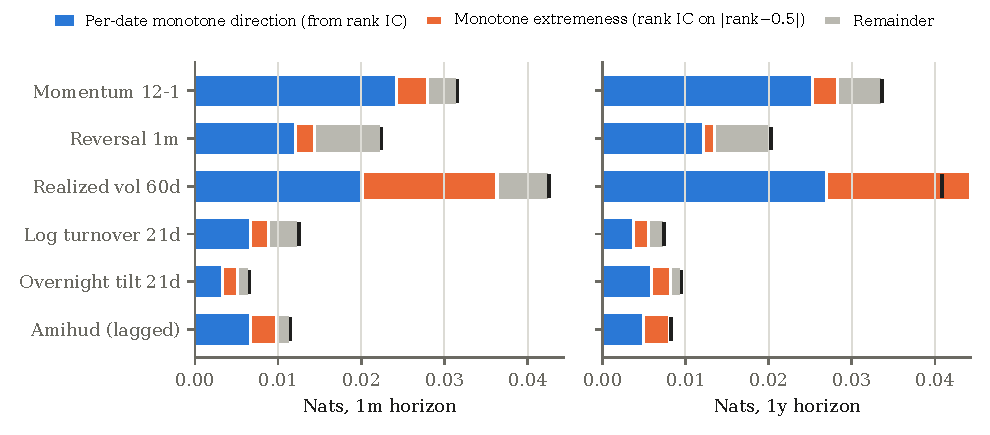
\includegraphics[width=\textwidth]{figures/fig2_accounting.pdf}
\caption{Approximate accounting for $\miex$ (black tick) at one month and one year:
MI implied by each month's rank IC (blue), by each month's extremeness rank IC
(orange), and the remainder (grey). Components use a Gaussian-copula conversion and
are not strictly additive.}
\label{fig:accounting}
\end{figure}

For signal research, a high MI score answers ``does this feature sort stocks by
future return in a typical month?'' and not ``in which direction, on average?''.
Ranking features on MI alone would place turnover and Amihud, whose average direction
is indistinguishable from zero, alongside features with a measurable average direction.

\subsection{Feature overlap: monotone and U-shaped}

\begin{figure}[t]
\centering
\begin{minipage}{0.5\textwidth}
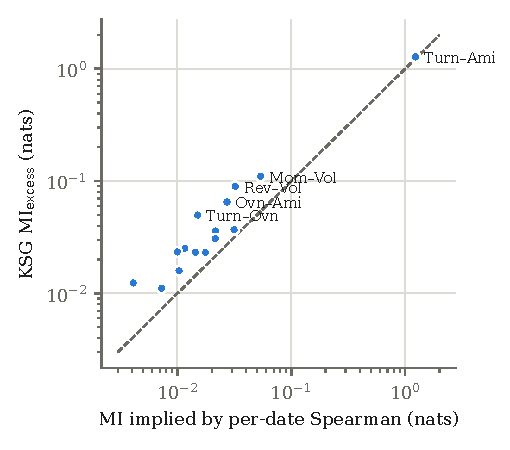
\includegraphics[width=\linewidth]{figures/fig4_redundancy.pdf}
\end{minipage}\hfill
\begin{minipage}{0.47\textwidth}
\caption{MI between pairs of features (vertical) against the MI implied by their
monthly Spearman correlation (horizontal), log scales. Points on the dashed line are
relationships rank correlation fully describes. Labelled points lie furthest above it.
Mom = momentum, Rev = reversal, Vol = volatility, Turn = turnover, Ovn = overnight
tilt, Ami = Amihud.}
\label{fig:redundancy}
\end{minipage}
\end{figure}

The same comparison between features (Figure~\ref{fig:redundancy}) separates two kinds
of overlap. Turnover and Amihud illiquidity are almost perfectly rank-correlated
($\rho = -0.950$); this is mechanical, since turnover is the denominator of Amihud's
measure. Their MI (1.27 nats) is within 4\% of what that correlation implies, so rank
correlation describes this overlap completely. (The original screen had blanked this
cell automatically because it exceeded a sanity ceiling; a follow-up check found no
tied values and confirmed the dependence was genuine.) By contrast, reversal and
volatility are uncorrelated on average ($\rho = -0.006$, 95\% interval
$[-0.050, 0.034]$) yet share 0.090 nats, 2.8 times the Gaussian-implied amount. A stock
that moved sharply in either direction last month tends to be a high-volatility stock:
a U-shaped relationship that correlation averages away. Momentum and volatility
($\rho = -0.105$, MI 0.110, 2.0 times implied) show the same pattern: extreme winners
and extreme losers both tend to be volatile. I have not checked these shapes with
binned conditional means, so ``U-shaped'' is the natural reading of the MI--correlation
gap rather than a fitted result. This is where MI earns its place next to correlation:
in revealing non-monotone structure between features, rather than in the case that
first motivated the analysis.

\subsection{Conditional MI: an apparent synergy and its correction}
\label{sec:cmi}

The first conditional run expressed each result as a survival ratio: conditional MI of
$A$ given $B$ divided by $A$'s marginal MI. All four pre-registered pairs returned
ratios above 100\% (117\%, 117\%, 128\% and 169\%), which would mean every feature
carries more information once its partner is known. A uniform result across unrelated
pairs is more likely an artifact than a market property, so three estimator checks
were run before interpretation:

\begin{itemize}
\item \textbf{Two estimators, two scales.} The numerator used the \texttt{npeet}
estimator and the denominator scikit-learn's. On identical inputs their marginal MI
estimates differed by a factor of 0.68--1.42 depending on the feature.
\item \textbf{Conditioning on noise is not neutral.} Conditioning a feature on a pure
random variable should leave its information unchanged. Instead the ``surviving''
fraction ranged from 44\% to 113\% across features, so the right benchmark is this
feature-specific value, not 100\%.
\item \textbf{Conditioning on itself does collapse.} Conditioning a feature on itself
left between $-8\%$ and $+6\%$, so the estimator can detect redundancy.
\end{itemize}

The corrected analysis uses one estimator throughout. For each date it computes $A$'s
permutation-corrected conditional information given $B$, and the same quantity with
$B$ replaced by random noise (averaged over 10 independent noise draws). With the same
estimator and inputs, conditioning on independent noise approximates $A$'s marginal
information $I(A;Y)$. The per-date difference therefore estimates
\[
I(A;Y\mid B) - I(A;Y),
\]
the interaction information of $A$, $B$ and $Y$ \citep{mcgill1954}. Negative values
indicate net redundancy (part of what $A$ says about $Y$ is already in $B$); positive
values indicate net synergy. The measure is net: it cannot separate redundancy from
synergy when both are present, which would require a partial-information
decomposition. Intervals bootstrap the per-date differences, so sampling variation in
both terms, including the benchmark, is carried into the interval. Before use, the
method was checked on synthetic data with a planted redundant pair (difference
$-0.106$ nats against a benchmark of $0.113$) and a planted additive pair ($+0.017$,
interval excluding zero).

\begin{table}[t]
\centering\small
\caption{Corrected conditional MI at the one-month horizon (nats). Benchmark: $A$'s
conditional information given random noise. Difference: given $B$ minus benchmark,
an estimate of interaction information. Re-run 2026-10-13; the original 2026-09
difference is shown for comparison.}
\label{tab:cmi}
\begin{tabular}{lrrrrcr}
\toprule
$A \mid B$ & Dates & Given $B$ & Benchmark & Difference & 95\% interval & Original \\
\midrule
Momentum $\mid$ volatility & 108 & 0.0349 & 0.0527 & $-0.0177$ & $[-0.0285, -0.0078]$ & $-0.0176$ \\
Volatility $\mid$ momentum & 108 & 0.0495 & 0.0697 & $-0.0202$ & $[-0.0305, -0.0096]$ & $-0.0199$ \\
Reversal $\mid$ momentum   & 108 & 0.0305 & 0.0335 & $-0.0030$ & $[-0.0113, \phantom{-}0.0052]$ & $-0.0025$ \\
Amihud $\mid$ turnover     & 127 & 0.0188 & 0.0206 & $-0.0018$ & $[-0.0107, \phantom{-}0.0068]$ & $-0.0013$ \\
\bottomrule
\end{tabular}
\end{table}

Table~\ref{tab:cmi} shows no synergy for any pair. Momentum and volatility show net
redundancy in both directions: as a ratio of point estimates, conditioning on
volatility lowers momentum's estimated information by about a third (0.018 of 0.053
nats), and conditioning on momentum lowers volatility's by about 29\%. No interval was
computed for these ratios, so they are descriptive. Each feature retains most of its
information, so this is partial overlap, not duplication. Reversal given momentum and
Amihud given turnover are inconclusive: their intervals include zero, which means
neither redundancy nor an independent increment is established. The Amihud result is
not at odds with the near-perfect correlation of the two features. Amihud's own
information about returns is small (0.023 nats), so there is little to remove, and the
interval is wide relative to it.

\section{Diagnostics}
\label{sec:repro}

\paragraph{Exact reproduction.} The 2026 re-run recomputed the screen from the same
panel and code with the original random seed. It reproduced all 30 point estimates and
date counts to floating-point precision (largest difference $10^{-16}$). The
conditional-MI differences reproduced within 0.0005 nats under newer library versions.
Reviewing the code during this exercise showed that the original driver set 15
permutations and 500 bootstrap draws after the functions had already fixed their
defaults, so the screen actually ran with 40 and 300; the effective values are reported
here.

\paragraph{Interval method and multiplicity (revision diagnostics).} Moving-block
intervals were 1--2\% wider than iid intervals at one week and one month, 10\% wider at
three and six months and 14\% wider at one year. With block lengths of 3, 6 and 12
months for every cell, only overnight tilt at three months changes conclusion (Section
4.1). The Holm adjustments in Section 4 were computed after the re-run from the
archived per-date series.

\paragraph{Estimator calibration.} Table~\ref{tab:cal} compares the
permutation-corrected KSG estimate with the known MI of bivariate Gaussian data at
$n=480$, the typical cross-section size. At moderate and strong dependence the estimate
is within 5\% of the truth, except at $\rho=0.3$, where it is 17\% high. At weak
dependence ($\rho\le0.2$, the range of most feature--return cells) the calibration is
imprecise: across 30 replications the estimate averaged 38--40\% of the true value,
with a standard error of about 0.004 nats. That shortfall is within noise at
$\rho=0.1$ and about three standard errors at $\rho=0.2$. Reported $\miex$ values for
weak cells may therefore understate the true MI.

\begin{table}[h]
\centering\small
\caption{KSG calibration on bivariate Gaussian data, $n=480$, 30 replications, 10
permutations each.}
\label{tab:cal}
\begin{tabular}{lrrrrrr}
\toprule
$\rho$ & 0.1 & 0.2 & 0.3 & 0.6 & 0.9 & 0.98 \\
\midrule
True MI (nats) & 0.0050 & 0.0204 & 0.0472 & 0.2231 & 0.8304 & 1.6145 \\
Estimated $\miex$ & 0.0020 & 0.0078 & 0.0550 & 0.2122 & 0.8472 & 1.6085 \\
SD across replications & 0.0195 & 0.0234 & 0.0307 & 0.0450 & 0.0616 & 0.0672 \\
\bottomrule
\end{tabular}
\end{table}

\paragraph{Reproducibility.} Table~\ref{tab:repro} lists the settings needed to
reproduce every number in the paper; a single notebook in the repository regenerates
them.

\begin{table}[h]
\centering\small
\caption{Run settings.}
\label{tab:repro}
\begin{tabularx}{\textwidth}{lX}
\toprule
Sample & Month-end rebalances 2010-01 to 2021-12 (144); 97--129 usable dates per cell; 464--490 stocks per date on average \\
MI estimator & KSG, $k=3$, scikit-learn 1.6.1; ranks scaled to $(0,1)$; 40 within-date permutations; seed 20260809 \\
Conditional MI & npeet-plus 0.2.0, $k=3$; 40 permutations for the conditional term; benchmark from 10 noise draws with 7 permutations each \\
Intervals & Circular moving-block bootstrap, 2,000 draws, blocks 3/3/3/6/12 months for 1w/1m/3m/6m/1y; seed 20260810 (original run: iid, 300 draws, 90\%) \\
Software & Python 3.13.16, NumPy 2.1.3, pandas 2.2.3 (re-run, 2026-10-13) \\
\bottomrule
\end{tabularx}
\end{table}

\section{Limitations and what this paper does not establish}

\begin{itemize}
\item \textbf{No trading claim.} The paper characterizes information. It forms no
portfolios, models no costs, and does not show that any feature is profitable.
\item \textbf{No mechanism.} The sign instability is documented, not explained; the
factor-exposure reading in Section~4.2 is untested. The U-shapes between features are
inferred from the MI--correlation gap, not fitted.
\item \textbf{Approximate accounting.} The Gaussian-copula conversion is an
approximation and the direction / extremeness / remainder shares are not an exact
decomposition.
\item \textbf{Net conditional measure, one horizon.} Interaction information is net of
redundancy and synergy. The four pairs were tested only at one month; conditional
estimation in three dimensions is noisier, and longer horizons were not pre-specified.
\item \textbf{Weak-dependence calibration.} Absolute MI values below about 0.02 nats
should be read as approximate.
\item \textbf{Calendar.} About 8\% of rebalance months were lost to closed or
incomplete dates in the panel index (Section~\ref{sec:data}); results will be
re-estimated on a corrected calendar.
\item \textbf{Universe approximation.} Membership comes from semi-annual snapshots,
including the truncated 2018-06-30 snapshot.
\end{itemize}

\section{Conclusion}

In Indian large- and mid-cap equities, permutation-corrected mutual information
indicates that all six common price and volume features sort the cross-section of
future returns, and this holds after a family-wise adjustment. Much of that
information, however, reflects relationships that are strong in a given month and
unstable in sign across months. Rank IC, by averaging signed values, answers the
question a portfolio needs answered; MI answers whether there is anything to condition
or time. Used between features, MI was most informative where correlation was weakest,
revealing that reversal and momentum are each related to volatility in a U-shape. And
conditional MI needed care: a single estimator and a feature-specific noise benchmark
turned an apparent uniform synergy into partial, net redundancy between momentum and
volatility. The procedural lesson is that a surprisingly uniform result is a reason to
test the estimator before interpreting the market.

\aistatement
\availability{\ghbase/indian-equity-research/tree/main/p3_mi_screen}

\bibliographystyle{plainnat}
\bibliography{../common/refs}

\end{document}
